\documentclass{article}
\usepackage[utf8]{inputenc}
\usepackage{amsmath}
\usepackage{graphicx}
  \DeclareGraphicsExtensions{.png, .jpeg}
\usepackage{caption}
\usepackage[top=1in, bottom=1in, left=1in, right=1in]{geometry}

\title{STAT 775: Machine Learning \\ Midterm}
\author{Terence Henriod}
\date{\today}

\begin{document}

\clearpage            % All of
\maketitle            % this,
\thispagestyle{empty} % removes the page number from the title page

\begin{abstract}
This take-home Midterm is due Wednesday at 1:00 p.m. at the beginning of class.
\end{abstract}

\newpage
\section{Problem 01}
\subsection{Problem Statement}
ESL Exercise 4.2:

\subsection{Solution}
\begin{enumerate}
  \item Recall that linear discriminant functions take the form
  $$\delta_{k}(x) = x^{T}\Sigma^{-1}\mu_{k} - \frac{1}{2}\mu_{k}^{T}\Sigma^{-1}\mu_{k} + log\pi_{k}$$
  and for classification we choose the class with the greatest discriminant for a given $x$. In the two class with the parameters as defined in the problem, in order to classify to class 2, we have $\delta_{2}(x) > \delta_{1}(x)$, so
  \begin{align*}
    x^{T}\Sigma^{-1}\mu_{2} - \frac{1}{2}\mu_{2}^{T}\Sigma^{-1}\mu_{2} + log\pi_{2} &> x^{T}\Sigma^{-1}\mu_{1} - \frac{1}{2}\mu_{1}^{T}\Sigma^{-1}\mu_{1} + log\pi_{1}\\
    x^{T}\Sigma^{-1}\mu_{2} - \frac{1}{2}\mu_{2}^{T}\Sigma^{-1}\mu_{2} &> x^{T}\Sigma^{-1}\mu_{1} - \frac{1}{2}\mu_{1}^{T}\Sigma^{-1}\mu_{1} + log\pi_{1} - log\pi_{2}\\
    x^{T}\Sigma^{-1}\mu_{2} &> x^{T}\Sigma^{-1}\mu_{1} + \frac{1}{2}\mu_{2}^{T}\Sigma^{-1}\mu_{2} - \frac{1}{2}\mu_{1}^{T}\Sigma^{-1}\mu_{1} + log\pi_{1} - log\pi_{2}\\
    x^{T}\Sigma^{-1}\mu_{2} - x^{T}\Sigma^{-1}\mu_{1} &> \frac{1}{2}\mu_{2}^{T}\Sigma^{-1}\mu_{2} - \frac{1}{2}\mu_{1}^{T}\Sigma^{-1}\mu_{1} + log\pi_{1} - log\pi_{2}\\
    x^{T}\Sigma^{-1}(\mu_{2} - \mu_{1}) &> \frac{1}{2}\mu_{2}^{T}\Sigma^{-1}\mu_{2} - \frac{1}{2}\mu_{1}^{T}\Sigma^{-1}\mu_{1} + log\pi_{1} - log\pi_{2}\\
  \end{align*}
  Now, since we have class sizes $N_{1}$ and $N_{2}$ with $N = N_{1} + N_{2}$, this means that $\pi_{k} = N_{k} / N$. This gives the final equation
  $$ x^{T}\Sigma^{-1}(\mu_{2} - \mu_{1}) > \frac{1}{2}\mu_{2}^{T}\Sigma^{-1}\mu_{2} - \frac{1}{2}\mu_{1}^{T}\Sigma^{-1}\mu_{1} + log(\frac{N_{1}}{N}) - log(\frac{N_{2}}{N}) $$

  \item I don't think I'm able to solve this one.

  \item In the previous problem statement, the assertion $ \hat{\Sigma_{B}} = (\hat{mu_{2}} - \hat{\mu_{1}})(\hat{mu_{2}} - \hat{\mu_{1}})^{T}$ is made, we can say that
  $$ \hat{\Sigma_{B}}\beta = (\hat{mu_{2}} - \hat{\mu_{1}})(\hat{mu_{2}} - \hat{\mu_{1}})^{T} $$
  which is equivalent to:
  $$ (\hat{mu_{2}} - \hat{\mu_{1}}) * k $$
  for some scalar $k$. Since $k$ is a scalar, $ (\hat{mu_{2}} - \hat{\mu_{1}}) * k $ will be in the same direction as $ (\hat{mu_{2}} - \hat{\mu_{1}}) $, just in a different direction.

  \item Our results thus far have used a distinct coding of the classes. So the previous result holds in that regard. As for the class codings being arbitrary, the encodings used in the problem statement seem arbitrary enough, so I would assume the result holds in this regard as well.  

  \item I don't think I'm able to solve this one.
\end{enumerate}

\newpage
\section{Problem 02}
\subsection{Problem Statement}
ESL Exercise 4.6:

\subsection{Solution}
\begin{enumerate}
  \item The problem statement allows the assumption that the data are separable, and in fact separable by some $\beta_{SEP}$. By Eq. 4.46 from the ESL book, in the notation of the problem, then $ y_{i}\beta_{SEP}^{T}z_{i} \ge D $ for some minimum distance from the decision boundary $D$ must hold. Since for any $\beta_{1}$ and $\beta_{0}$ (which compose $\beta_{SEP}$) that satisfy the inequality, any positively scaled such $\beta$s will satisfy the inequality also. Thus we can choose some scaling factor $\rho$ s.t. $ \rho * D = 1$, there must exist a 
  $\beta_{SEP} = \beta_{SEP}\prime * \rho$ ($\beta_{SEP}\prime$ is some other, acceptable solution) s.t.:
  $$ y_{i}\beta_{SEP}^{T}z_{i} \ge 1 $$

  \item First, to show that the inequality holds:
  \begin{align*}
    ||\beta_{new} - \beta_{sep}||^{2} 
      &= ||\beta_{new}||^{2} + ||\beta_{sep}||^{2} - 2\beta_{sep}^{T}\beta_new \\
    &= ||\beta_{old} + y_{i}z_{i}||^{2} + ||\beta_{sep}||^{2} - 2\beta_{sep}^{T}(\beta_{old} + y_{i}z_{i}) \\
    &= ||\beta_{old}||^{2} + ||y_{i}z_{i}||^{2} + 2\beta_{old}^{T}y_{i}z_{i} + ||\beta_{sep}||^{2} - 2\beta_{sep}^{T}(\beta_{old} + y_{i}z_{i}) \\
    &= ||\beta_{old}||^{2} + 1 + 2\beta_{old}^{T}y_{i}z_{i} + ||\beta_{sep}||^{2} - 2\beta_{sep}^{T}(\beta_{old} + y_{i}z_{i}) \\
    &= ||\beta_{old}||^{2} + 2\beta_{old}^{T}y_{i}z_{i} + ||\beta_{sep}||^{2} - 2\beta_{sep}^{T}\beta_{old} - 2y_{i}\beta_{sep}^{T}z_{i} + 1\\
    &\le ||\beta_{old}||^{2} + 2\beta_{old}^{T}y_{i}z_{i} + ||\beta_{sep}||^{2} - 2\beta_{sep}^{T}\beta_{old} - 2 + 1\\
    &\le ||\beta_{old}||^{2} + ||\beta_{sep}||^{2} + 2\beta_{old}^{T}y_{i}z_{i} - 2\beta_{sep}^{T}\beta_{old} - 1 \\
    &\le ||\beta_{old} - \beta_{sep}||^{2} - 1 \\
  \end{align*}
  using $y_{i}\beta_{sep}^{T}z_{i} \ge 1$ from the previous part of the exercise. Also, in the previous exercise, because the result $y_{i}\beta_{sep}^{T}z_{i} \ge 1$ indicated a maximum separation distance, we could say that $2\beta_{old}^{T}y_{i}z_{i} \le y_{i}\beta_{sep}^{T}z_{i} $ and so that term is dwarfed by the 
  $-2\beta_{sep}^{T}\beta_{old}$ term, dropping it from the equation. This result means that the inequality
  \begin{align*}
  ||\beta_{old} - \beta_{sep}||^{2} + 2\beta_{old}^{T}y_{i}z_{i} - 1 &\le ||\beta_{old} - \beta_{sep}||^{2} - 1 \\
  ||\beta_{new} - \beta_{sep}||^{2} &\le ||\beta_{old} - \beta_{sep}||^{2} - 1
  \end{align*}
  must hold. \\

  Second, if we are to reach a solution, then $||\beta_{old} - \beta_{sep}||^{2} = 0$ at some point. By the previous result, each iteration improves our $\beta$ solution by at least $1$ each time. Suppose we start at some $\beta$ $\beta_{start}$, where $||\beta_{start} - \beta_{sep}||^{2} = i$. Since the algorithm improves the solution and reduces $i$ by $1$ with each iteration, we will reach a $\beta_{new} = \beta_{sep}$ in $i$ or fewer iterations.
\end{enumerate}


\newpage
\section{Problem 03}
\subsection{Problem Statement}
Build a logistic resgression classifier for the South African Heart Disease data and compare its performance with a neural network with one hidden layer.

\subsection{Results}
The results were somewhat disappointing. Neither classifier offered particularly good performance, and the neural net only got the performance it did by classifying everyithing as the most likely class. (I hope this was just the nature of the data and not because I forgot to do perform some technique or operation correctly). The results use a neural net with a hidden layer with 3 units, but increasing the number of hidden units produces the same result. Even dimensionality reduction techniques did not seem to help much. Shuffling the data proved only slightly helpful. As we discussed, the neural net should never under-perform logistic regression since LR is a subset of the neural network approach.

The confusion matrices were as follows.\\
For LR:\\
\newline
\begin{tabular}{| c || c | c | c |}
  \hline
  Actual / Predicted & No CHD & CHD & \% Correct \\
  \hline
  \hline
  No CHD             &     90 &  17 &         84 \\
  \hline
  CHD                &     16 &  31 &         66 \\
  \hline
  \hline
  Overall            &        &     &         79 \\
  \hline
\end{tabular}
%
%
\hfill\newline\hfill\\
For Neural Net:\\
\begin{tabular}{| c || c | c | c |}
  \hline
  Actual / Predicted & No CHD & CHD & \% Correct \\
  \hline
  \hline
  No CHD             &    107 &     &        100 \\
  \hline
  CHD                &     47 &     &          0 \\
  \hline
  \hline
  Overall            &        &     &         69 \\
  \hline
\end{tabular}

\subsection{Code}
\begin{verbatim}
#
# Initial Setup
#
setwd("C:/Users/Terence/Documents/GitHub/STAT775/Midterm/")
# setwd("~/STAT775/HW03/")

DATA.FILE.NAME <- "../DataSets/south.african.heart.disease/data.disease"


#
# Data Handling
#
shuffle.data <- function(x) {
  # x: a numeric matrix

  for (i in 1:nrow(x)) {
    one <- round(runif(1, 1, nrow(x)))
    other <- round(runif(1, 1, nrow(x)))

    temp <- x[one, ]
    x[one, ] <- x[other, ]
    x[other, ] <- temp
  }

  return(x)
}

code.data <- function(dat.a) {
  family.history <- rep(0.0, nrow(dat.a))

  data <- data.frame(dat.a[, 1:4], family.history, dat.a[6:10])

  for (i in 1:nrow(data)) {
    if (dat.a[i, 'famhist'] == 'Present') {
      data[i, 'family.history'] <- 1.0
    }
  }

  return(shuffle.data(data.matrix(data)))
}

get.data.tuples <- function(data) {
  last.column <- ncol(data)

  return(list(
    observations = (data.matrix(data[, -last.column])),
    targets = data.matrix(data[, last.column])
  ))
}


#
# Logistic Regression
#
logistic.predict <- function(x, b) {
  #
  # Args:
  #   x: a p x 1 column vector of observation values
  #   b: a p X 1 column vector of model weights (betas)

  e <- exp(matrix(b, nrow = 1) %*% rbind(1.0, matrix(x, ncol = 1)))
  return(e / (1.0 + e))
}

newton.raphson.iteration <- function(X, y, old.betas, step.size = 0.5) {
  #
  # Args:
  #   X: N x p matrix of observations
  #   y: column vector of N target labels
  #   old.betas: column vector of (p + 1) model parameters
  #   step.size: a rate controlling parameter

  p <- matrix(0, nrow = nrow(y), ncol = 1)
  for (i in 1:nrow(y)) {
    p[i, 1] <- logistic.predict(x = data.matrix(X[i, ]), b = old.betas)
  }

  W <- diag(1, nrow(y), nrow(y))
  for (i in 1:nrow(y)) {
    W[i, i] <- p[i, 1] * (1.0 - p[i, 1])
  }

  X.b <- cbind(1.0, X)  # X with 1s prepended for bias term

  z <- (X.b %*% old.betas) +
    (solve(W + diag(0.001, nrow(W), ncol(W))) %*% (y - p))

  step <- solve((t(X.b) %*% W %*% X.b) + diag(0.001, ncol(X.b), ncol(X.b))) %*%
    t(X.b) %*% (y - p)
  step <- step * step.size

  return(old.betas + step)
}

train.logistic.model <- function(X, y, n.iterations = 400, step.size = 0.2) {
  #
  # Args:
  #   X: N x p matrix of observations, observations are rows
  #   y: N x 1 column vector of class labels {0, 1}
  #   n.iterations: the number of approximation iterations to perform
  #   step.size: used to slow the rate of convergence to prevent overshooting

  # start with model parameters at 0 - arbitrary starting point
  betas <- matrix(0, nrow = ncol(X) + 1, 1)

  # iterate until parameter updates become arbitrarily small
  old.betas <- betas + 1.0
  i <- 0
  while (i < n.iterations) {
    betas <- newton.raphson.iteration(
      X = X,
      y = y,
      old.betas = betas,
      step.size = step.size
    )

    # TODO: use method for finding convergence, not just arbitrary iterations

    i <- i + 1
  }

  return(betas)
}


#
# Neural Net
#
sigmoid <- function(x) {
  #
  # Args:
  #   x: a numeric or vector; the function is applied element-wise

  return(1.0 / (1.0 + exp(-x)))
}

sigmoid.derivative <- function(x) {
  #
  # Args:
  #   x: a numeric or vector

  return(sigmoid(x) * (1.0 - sigmoid(x)))
}

construct.neural.net <- function(
  topology = c(2, 2, 1),
  activation = sigmoid,
  activation.derivative = sigmoid.derivative,
  debug = F) {
  #
  # Args:
  #   topology: a list or vector of the dimensions of each layer
  #   activation: a function to be used for the activation of each unit
  #   activation.derivative: a function that is the derivative of activation

  layer.weights <- list()
  derivative.matrices <- list()
  outputs <- list()

  previous.layer.dim <- 1
  next.layer.dim <- 1
  for (i in 1:(length(topology) - 1)) {
    previous.layer.dim <- topology[[i]] + 1  # +1 for bias
    next.layer.dim <- topology[[i + 1]]
    num.elements <- (previous.layer.dim) * next.layer.dim

    layer.weights[[i]] <- matrix(
      if(debug) {rep(1, num.elements)}
      else {runif(n = num.elements, min = -0.001, max = 0.001)},
      nrow = previous.layer.dim,
      ncol = next.layer.dim
    )

    outputs[[i]] <- matrix(0, nrow = next.layer.dim, ncol = 1)
    derivative.matrices[[i]] <- diag(0, next.layer.dim)
  }

  return(list(
    input.dim = topology[[1]],
    output.dim = next.layer.dim,  # should be dim of last layer
    n.layers = length(layer.weights),
    activation = activation,
    activation.deriv = activation.derivative,
    input = matrix(0, nrow = 1, ncol = topology[[1]]),
    output = matrix(0, nrow = tail(topology, 1)[[1]], 1),
    weights = layer.weights,
    outputs = outputs,
    derivatives = derivative.matrices
  ))
}

apply.inputs <- function(net, x, for.training = T) {
  #
  # Args:
  #   x: a 1 x n vector of inputs; n should be the same as for net
  #   net: a structure with all of the appropriate data for a neural network,
  #        as created by construct.neural.net()
  #   for.training[T]: currently unused

  net$input <- matrix(x, nrow = 1)
  previous.output <- cbind(net$input, 1)
  for (i in 1:net$n.layers) {
    weighted.sums <- previous.output %*% net$weights[[i]]

    net$outputs[[i]] <- net$activation(weighted.sums)

    net$derivatives[[i]] <- diag(
      as.list(net$activation.deriv(weighted.sums)),
      length(net$outputs[[i]])
    )

    previous.output <- cbind(net$outputs[[i]], 1)
  }

  net$output <- t(tail(net$outputs, 1)[[1]])

  return(net)
}

backprop.weight.update <- function(net, target, learning.rate = 2) {
  #
  # Args:
  #   net: a neural net object that has had inputs applied and derivatives stored
  #   target: a column vector; the target output that should have been observed
  #   learning.rate: the learning rate of the network
  #                  TODO: refactor learning.rate to be less hacky, allow for
  #                        advanced techniques

  last.index <- net$n.layers

  deltas <- list()
  error <- matrix(net$output, ncol = 1) - matrix(target, ncol = 1)
  deltas[[last.index + 1]] <- error
  W <- diag(1, nrow = nrow(error))
  D <- net$derivatives[[last.index]]
  for (i in last.index:1) {
    deltas[[i]] <- D %*% W %*% deltas[[i + 1]]

    if (i > 1) {
      D <- net$derivatives[[i - 1]]
      W <- net$weights[[i]]
      W <- W[1:(nrow(W) - 1), ]
    }
  }

  weight.updates <- list()
  o.hat <- cbind(net$input, 1)
  for (i in 1:last.index) {
    weight.updates[[i]] <- -learning.rate * t(deltas[[i]] %*% o.hat)

    if (i < last.index) {
      o.hat <- cbind(net$outputs[[i]], 1)
    }
  }

  for (i in 1:length(weight.updates)) {
    net$weights[[i]] <- net$weights[[i]] + weight.updates[[i]]
  }

  return(net)
}


######
# MAIN
######
data.fram.e <- read.table(
  "http://www-stat.stanford.edu/~tibs/ElemStatLearn/datasets/SAheart.data",
  sep = ",",
  head = T,
  row.names = 1
)
data <- code.data(data.fram.e)
boundary <- 2 * nrow(data) / 3
train <- get.data.tuples(data[1:boundary, ])
test <- get.data.tuples(data[-(1:boundary), ])

# Logistic
logistic.model <- train.logistic.model(X = train$observations, y = train$targets)

logistic.confusion <- matrix(0, nrow = 3, ncol = 3)
for (i in 1:nrow(test$targets)) {
  prediction <- round(logistic.predict(x = test$observations[i, ], b = logistic.model))
  label <- test$targets[[i]]

  logistic.confusion[label + 1, prediction + 1] <-
    logistic.confusion[label + 1, prediction + 1] + 1
}


# Neural Net
NUM.EPOCHS <- 700
chd.net <- construct.neural.net(
  topology = c(9, 3, 1),
  activation = sigmoid,
  activation.deriv = sigmoid.derivative
)

for (t in 1:NUM.EPOCHS) {
  for (i in 1:nrow(train$targets)) {
    chd.net <- apply.inputs(
      net = chd.net,
      x = matrix(train$observations[i, ], nrow = 1)
    )
    chd.net <- backprop.weight.update(
      net = chd.net,
      target = matrix(train$targets[i, ], ncol = 1),
      learning.rate = 0.2
    )
  }
}

net.confusion <- matrix(0, 3, 3)
for (i in 1:nrow(test$observations)) {
  prediction <- round(
    apply.inputs(
      net = chd.net,
      x = matrix(test$observations[i, ], nrow = 1),
      for.training = F
    )$output
  )

  label <- test$targets[[i]]

  net.confusion[label + 1, prediction + 1] <-
    net.confusion[label + 1, prediction + 1] + 1
}

# Results
compute.confusion.percentages <- function(confusion) {
  rownames(confusion) <- c('Actual No CHD', 'Actual CHD', '%.Correct')
  colnames(confusion) <- c('Actual No CHD', 'Actual CHD', '%.Correct')

  row.sums <- rowSums(confusion)
  col.sums <- colSums(confusion)
  correct <- 0
  for (i in 1:2) {
    confusion[i, 3] <- confusion[i, i] / row.sums[[i]]
    confusion[3, i] <- confusion[i, i] / col.sums[[i]]
    correct <- correct + confusion[i, i]
  }
  confusion[[3,3]] <- correct / sum(row.sums)

  return(confusion)
}

logistic.confusion <-compute.confusion.percentages(logistic.confusion)
net.confusion <-compute.confusion.percentages(net.confusion)
print(logistic.confusion, digits = 2)
print(net.confusion, digits = 2)
\end{verbatim}


\newpage
\section{Problem 03}
\subsection{Problem Statement}
Build a two classifiers for lpsa in the prostate data base. Compare the performance of linear regresssion against a neural network with a hidden layer (scale the output).

\subsection{Results}
Once again the neural net was outperformed. This could be because I did not ``scale the outputs" properly (I was unsure about how to go about this), or because the nerual net is too simple to be effective.

I was not sure how to present the results, so here are some screenshots of various R output indicating a comparison of the Residual Sum of Squares (RSS) for each method and example comparisons:

\begin{figure}[h!]
  \centering
  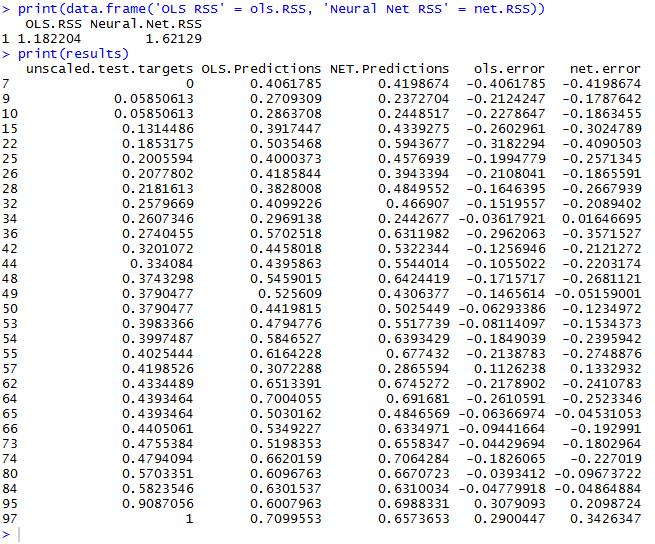
\includegraphics[width=.8\linewidth]{Problem_04_results}
  \caption{Error results for the logistic regression and neural net models.}
  \label{fig:P04_results}
\end{figure}

\subsection{Code}
\begin{verbatim}
#
# Initial Setup
#
setwd("C:/Users/Terence/Documents/GitHub/STAT775/HW03/")
DATA.FILE.NAME <- "../DataSets/prostate_cancer/prostate_cancer_data"

#
# Data Handling
#
# these include the intercept that gets added to the matrices
FEATURE.INDICES <- 1:9
TARGET.INDEX <- 10
TRAIN.SET.FLAG <- 11

scale.outputs <- function(x) {
  # Args:
  #  x: a numerical vector, column or row

  range <- max(x) - min(x)
  scaled.x <- (x - min(x)) / range
  return(scaled.x)
}

unscale.outputs <- function(x, max.unscaled, min.unscaled) {
  range <- max.unscaled - min.unscaled
  return((x * range) + min.unscaled)
}


data <- read.table(DATA.FILE.NAME)
# according to the dataset info, this needs to be done
data[, 1:8] <- scale(data[, 1:8], T, T)
intercept <- rep(1, nrow(data))
data <- data.frame(Intercept = intercept, data)

# store data with rows as observations
train.data <- data.matrix(subset(data, data$train == T))[, FEATURE.INDICES]
train.targets <- data.matrix(subset(data, data$train == T))[, TARGET.INDEX]

test.data <- data.matrix(subset(data, data$train == F))[, FEATURE.INDICES]
test.targets <- data.matrix(subset(data, data$train == F))[, TARGET.INDEX]

max.test.target <- max(test.targets)
min.test.target <- min(test.targets)
unscaled.test.targets <- test.targets

train.targets <- scale.outputs(train.targets)
test.targets <- scale.outputs(test.targets)

#
# Regression
#
ols.regression <- function(x, y) {
  #
  # Args:
  #   x: a matrix of observations; each observation is stored as a row
  #   y: a column vector of the targets, or actual value/label, for each
  #      observation

  return(list(
    beta.hat = solve(t(x) %*% x) %*% t(x) %*% matrix(y, ncol = 1)
  ))
}

ols.predict <- function(model, x) {
  #
  # Args:
  #   model: an n x 1 column vector of regression coefficients
  #   x: a ? x n matrix of observation data

  return(t(model$beta.hat) %*% t(x))
}



#
# Neural Net
#

sigmoid <- function(x) {
  #
  # Args:
  #   x: a numeric or vector; the function is applied element-wise

  return(1.0 / (1.0 + exp(-x)))
}

sigmoid.derivative <- function(x) {
  #
  # Args:
  #   x: a numeric or vector

  return(sigmoid(x) * (1.0 - sigmoid(x)))
}

construct.neural.net <- function(
  topology = c(2, 2, 1),
  activation = sigmoid,
  activation.derivative = sigmoid.derivative,
  debug = F) {
  #
  # Args:
  #   topology: a list or vector of the dimensions of each layer
  #   activation: a function to be used for the activation of each unit
  #   activation.derivative: a function that is the derivative of activation

  layer.weights <- list()
  derivative.matrices <- list()
  outputs <- list()

  previous.layer.dim <- 1
  next.layer.dim <- 1
  for (i in 1:(length(topology) - 1)) {
    previous.layer.dim <- topology[[i]] + 1  # +1 for bias
    next.layer.dim <- topology[[i + 1]]
    num.elements <- (previous.layer.dim) * next.layer.dim

    layer.weights[[i]] <- matrix(
      if(debug) {rep(1, num.elements)}
      else {runif(n = num.elements, min = -0.001, max = 0.001)},
      nrow = previous.layer.dim,
      ncol = next.layer.dim
    )

    outputs[[i]] <- matrix(0, nrow = next.layer.dim, ncol = 1)
    derivative.matrices[[i]] <- diag(0, next.layer.dim)
  }

  return(list(
    input.dim = topology[[1]],
    output.dim = next.layer.dim,  # should be dim of last layer
    n.layers = length(layer.weights),
    activation = activation,
    activation.deriv = activation.derivative,
    input = matrix(0, nrow = 1, ncol = topology[[1]]),
    output = matrix(0, nrow = tail(topology, 1)[[1]], 1),
    weights = layer.weights,
    outputs = outputs,
    derivatives = derivative.matrices
  ))
}

apply.inputs <- function(net, x, for.training = T) {
  #
  # Args:
  #   x: a 1 x n vector of inputs; n should be the same as for net
  #   net: a structure with all of the appropriate data for a neural network,
  #        as created by construct.neural.net()
  #   for.training[T]: currently unused

  net$input <- matrix(x, nrow = 1)
  previous.output <- cbind(net$input, 1)
  for (i in 1:net$n.layers) {
    weighted.sums <- previous.output %*% net$weights[[i]]

    net$outputs[[i]] <- net$activation(weighted.sums)

    net$derivatives[[i]] <- diag(
      as.list(net$activation.deriv(weighted.sums)),
      length(net$outputs[[i]])
    )

    previous.output <- cbind(net$outputs[[i]], 1)
  }

  net$output <- t(tail(net$outputs, 1)[[1]])

  return(net)
}

backprop.weight.update <- function(net, target, learning.rate = 2) {
  #
  # Args:
  #   net: a neural net object that has had inputs applied and derivatives stored
  #   target: a column vector; the target output that should have been observed
  #   learning.rate: the learning rate of the network
  #                  TODO: refactor learning.rate to be less hacky, allow for
  #                        advanced techniques

  last.index <- net$n.layers

  deltas <- list()
  error <- matrix(net$output, ncol = 1) - matrix(target, ncol = 1)
  deltas[[last.index + 1]] <- error
  W <- diag(1, nrow = nrow(error))
  D <- net$derivatives[[last.index]]
  for (i in last.index:1) {
    deltas[[i]] <- D %*% W %*% deltas[[i + 1]]

    if (i > 1) {
      D <- net$derivatives[[i - 1]]
      W <- net$weights[[i]]
      W <- W[1:(nrow(W) - 1), ]
    }
  }

  weight.updates <- list()
  o.hat <- cbind(net$input, 1)
  for (i in 1:last.index) {
    weight.updates[[i]] <- -learning.rate * t(deltas[[i]] %*% o.hat)

    if (i < last.index) {
      o.hat <- cbind(net$outputs[[i]], 1)
    }
  }

  for (i in 1:length(weight.updates)) {
    net$weights[[i]] <- net$weights[[i]] + weight.updates[[i]]
  }

  return(net)
}


######
# MAIN
######
ols.model <- ols.regression(x = train.data, y = train.targets)
predictions <- ols.predict(model = ols.model, x = test.data)
OLS.Predictions <- as.list(predictions)
# OLS.Predictions <- as.list(unscale.outputs(predictions, max.test.target, min.test.target))

ols.RSS <- sum((test.targets - predictions) ^ 2)
print(ols.RSS)


# Neural Net
NUM.EPOCHS <- 1000
prostate.net <- construct.neural.net(
  topology = c(ncol(train.data), 10, 1),
  activation = sigmoid,
  activation.deriv = sigmoid.derivative
)

for (t in 1:NUM.EPOCHS) {
  for (i in 1:length(train.targets)) {
    prostate.net <- apply.inputs(
      net = prostate.net,
      x = matrix(train.data[i, ], nrow = 1)
    )
    prostate.net <- backprop.weight.update(
      net = prostate.net,
      target = matrix(train.targets[[i]], ncol = 1),
      learning.rate = 0.2
    )
  }
}

net.RSS <- 0
net.predictions <- list()
for (i in 1:length(test.targets)) {
  prostate.net <- apply.inputs(
    net = prostate.net,
    x = matrix(test.data[i, ], nrow = 1)
  )

  net.predictions[[i]] <- prostate.net$output

  error.squared <- (prostate.net$output - test.targets[[i]]) ^ 2

  net.RSS <- net.RSS + error.squared
}
NET.Predictions <- as.list(net.predictions)
# NET.Predictions <- as.list(unscale.outputs(unlist(net.predictions), max.test.target, min.test.target))

unscaled.test.targets <- test.targets

ols.error <- list()
net.error <- list()
for (i in 1:length(unscaled.test.targets)) {
  ols.error[[i]] <- unscaled.test.targets[[i]] - OLS.Predictions[[i]]
  net.error[[i]] <- unscaled.test.targets[[i]] - NET.Predictions[[i]]
}

results <- data.frame(
  cbind(
    unscaled.test.targets,
    OLS.Predictions,
    NET.Predictions,
    ols.error,
    net.error
  )
)

print(data.frame('OLS RSS' = ols.RSS, 'Neural Net RSS' = net.RSS))
print(results)
\end{verbatim}

\end{document}
